\chapter{Dritter Anhang - Aufbau des SGAM Frameworks}
\label{Kap:SGAM_aufbau}

\section{Grundlegender Aufbau des SGAM Frameworks}
	Das \ac{SGAM} besteht aus Interoperabilitäts-Ebenen (Layers), physikalischen Domänen (Domains) entlang der Energieumwandlungskette und funktionaler Zonen (Zones) des Prozessmanagements, die in Abb. \ref{Abb:SGAM} dargestellt werden.  Jede Funktionseinheit (entity) einer Smart Grid Anwendung kann von einer architektonischen Perspektive einer der SGAM Layers, Domains und Zones zugeordnet werden.

	\begin{figure}[h]
		\centering
		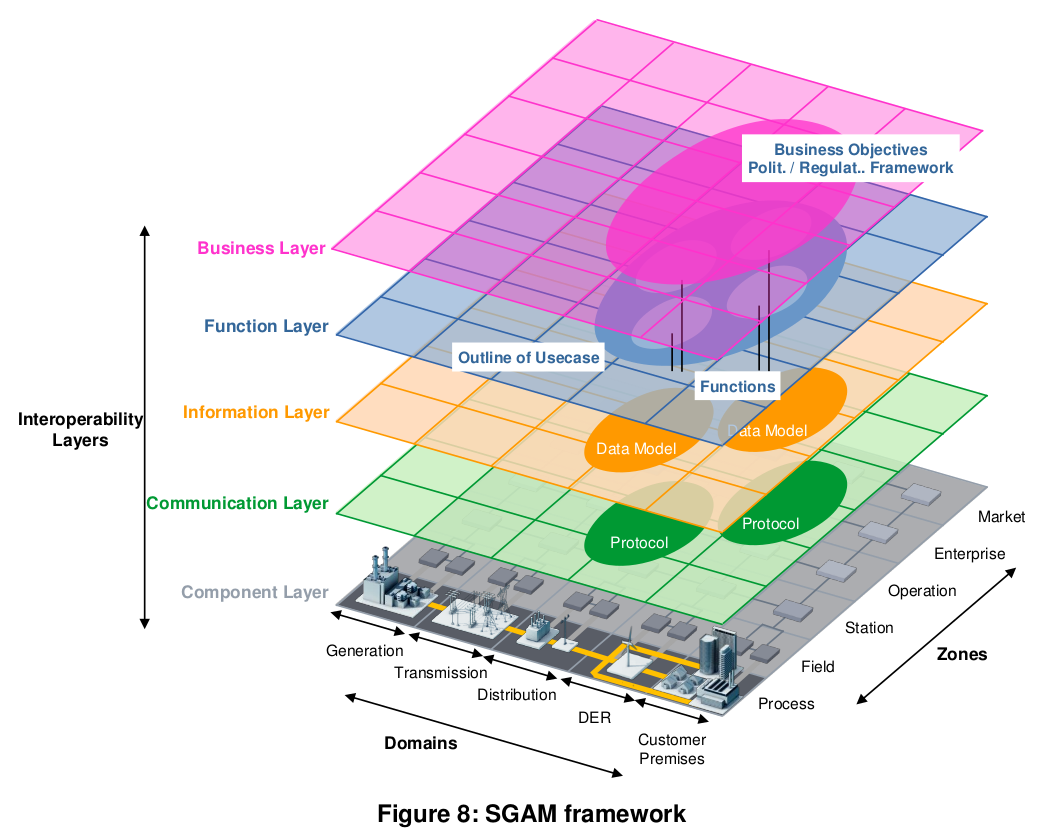
\includegraphics[width=14cm]{SGAM}
		\caption{SGAM framework \cite{CENELEC_SmartGrid}}
		\label{Abb:SGAM}
	\end{figure}
	
	\section{SGAM Tabellen}
	
	\paragraph{SGAM Interoperabilitäts-Ebenen (Interoperability Layers)}
		Die in Abbildung \ref{Abb:SGAM} gezeigten, dem SGAM zugrunde liegenden, Interoperabilitäts-Ebenen (Layers) werden in Tabelle \ref{Tab:SGAM_Layers} definiert.		
	
	\paragraph{SGAM Smart Grid Plane}
		Im Allgemeinen kann bei Energiemanagementsystemen zwischen den beiden Gesichtspunkten des elektrischen Prozesses und des Prozessmanagements unterschieden werden. Im SGAM wird beides in der Smart Grid Plane dargestellt. Der Prozess der Energiewandlungskette von der Erzeugung über die Umwandlung und Verteilung bis hin zum Verbrauch im Smart Grid wird einzelnen physikalischen Domänen (Domains) zugeordnet und das Prozessmanagement hierarschisch aufgebauten Zonen (Zones). \\
	
	\paragraph{SGAM Domänen (Domains)}		
		Die in Tabelle \ref{Tab:SGAM_Domains} beschriebenen SGAM Domänen decken die gesamte Energiewandlungskette in einem Smart Grid ab. 
	
	\paragraph{SGAM Zonen (Zones)}
		Die in Tabelle \ref{Tab:SGAM_Zones} beschriebenen funktional separierten SGAM Zonen spiegeln ein hierarchisches Modell wider, das sowohl den Prozess als auch das Prozessmanagement umfasst. 
	
		\begin{table}
			\begin{tabularx}{\linewidth}{|c|X|}
				\hline 
				\textbf{Ebene} 				& \textbf{Beschreibung}   \\ 
				\hline 
				Business 				& Repräsentiert den unternehmerischen Blickwinkel auf den Austausch Smart Grid zugehöriger Informationen. Diese Ebene kann regulatorische und ökonomische (Markt-)Strukturen und Richtlinien, Geschäftsmodelle, -optionen und -prozesse, sowie Geschäfts-Portfolios (Produkte und Dienstleistungen) beteiligter Marktteilnehmer*innen beinhalten. \\
				\hline 
				Funktion 		& Beschreibt Funktionen und Dienste inklusive deren Beziehung von einem architektonischen Blickpunkt aus. Die Funktionen werden unabhängig von Aktoren und physikalischen Implementierungen in Anwendungen, System und Komponenten dargestellt und von der Aktoren unabhängigen Use Case Funktionalität abgeleitet. \\
				\hline
				Information		& Beschreibt die Information, die von Funktionen verwendet und zwischen Funktionen, Diensten und Komponenten ausgetauscht wird. Es beinhaltet Informationsobjekte und die zugrunde liegenden kanonischen Datenmodelle und definiert damit die übliche Semantik für Funktionen und Dienste, um den interoperablen Austausch von Information mit Kommunikationsmitteln zu ermöglichen. \\
				\hline
				Kommunikation		 			& Beschreibt Protokolle und Mechanismen für den interoperablen Austausch von Informationen zwischen Komponenten im Kontext des zugrunde liegenden Anwendungsfall, Funktion oder Service und zugehöriger Informationsobjekte oder Datenmodelle. \\
				\hline
				Komponenten 			& Schreibt die physikalische Aufteilung aller beteiligten Komponenten im Smart Grid Kontext. Das beinhaltet System-Akteure, Anwendungen, Geräte zur Energieversorgung, Schutz, Geräte zur Fernsteuerung, Netzwerkinfrastruktur (verkabelte und kabellose Kommunikation, Router, Switches, Server) und jegliche Art von Computern.  \\
				\hline 
				
			\end{tabularx}
			\caption{SGAM Ebenen (Layers) eines Energiesystems \\ nahezu unverändert aus dem Englischen übersetzt \cite[S.27]{CENELEC_SmartGrid}}
			\label{Tab:SGAM_Layers}
		\end{table}	

		\begin{table}
			\begin{tabularx}{\linewidth}{|c|X|}
				\hline 
				\textbf{Domäne} 				& \textbf{Beschreibung}   \\ 
				\hline 
				Bulk 				& Repräsentiert die Erzeugung elektrischer Energie in großen \\
				Generation			&  Mengen wie z.B. durch fossile, nukleare und wasserbetriebene Kraftwerke, Off-shore Windparks und große Solarkraftwerke. \\
				\hline 
				Transmission 		& Repräsentiert die Infrastruktur und Organisation für den Transport elektrischer Energie über weite Distanzen. \\
				\hline
				Distribution		& Repräsentiert die Infrastruktur und Organisation für die Verteilung von elektrischer Energie zu Verbraucher*innen. \\
				\hline
				DER		 			& Repräsentiert verteilte elektrische Ressourcen (distributed electric resource) mit Energieerzeugungstechnologien im kleinen Maßstab (typ. von 3~kW bis 10.000~kW), die direkt ans öffentliche Stromnetz angeschlossen sind. \\
				\hline
				Customer 			& Beinhaltet sowohl den Endverbrauch von Elektrizität als auch  \\
				Premises			& elektrische Energieerzeugung z.B. in Form von PV-Anlagen, Batterien, Mikro-Turbinen, etc.. Die Räumlichkeiten (Premises) umfassen industrielle, kommerzielle und häusliche Anlagen.\\
				\hline 
			\end{tabularx}
			\caption{SGAM Domänen (Domains) eines Energiesystems}
			\label{Tab:SGAM_Domains}
		\end{table}	
		

		\begin{table}
			\begin{tabularx}{\linewidth}{|c|X|}
				\hline 
				\textbf{Zone} & \textbf{Beschreibung}   \\ 
				\hline 
				Process 	& Beinhaltet die physikalische, chemische oder räumliche Transformation von Energie und die direkt involvierten Gerätschaften. \\ 
				\hline 
				Field 		&  Beinhaltet Geräte für Schutz, Steuerung und Überwachung des Prozesses des Energiesystems. \\
				\hline
				Station 	& Repräsentiert die räumliche Agglomeration für die Field Zone. \\
				\hline
				Operation 	& Beinhaltet Steuerungsoperationen für das Energiesystem. \\
				\hline
				Enterprise 	& Beinhaltet kommerzielle und organisatorische Prozesse, Services und Infrastrukturen für Unternehmen. \\
				\hline
				Market 		& Stellt die möglichen Markthandlungen dar entlang der Energiewandlungskette.\\
				\hline 
			\end{tabularx} 
			\caption{SGAM Zonen (Zones)}
			\label{Tab:SGAM_Zones}
		\end{table}	
					
	\section{Überblick einer Beispiel Einordnung ins SGAM }
		Die Abbildung \ref{Abb:SGAM_map_overview} zeigt die einzelnen Schritte bei der Erstellung des SGAM Modells in Kapitel \ref{Kap:Konzept_func}.
		\begin{figure}[h] 
			\centering
			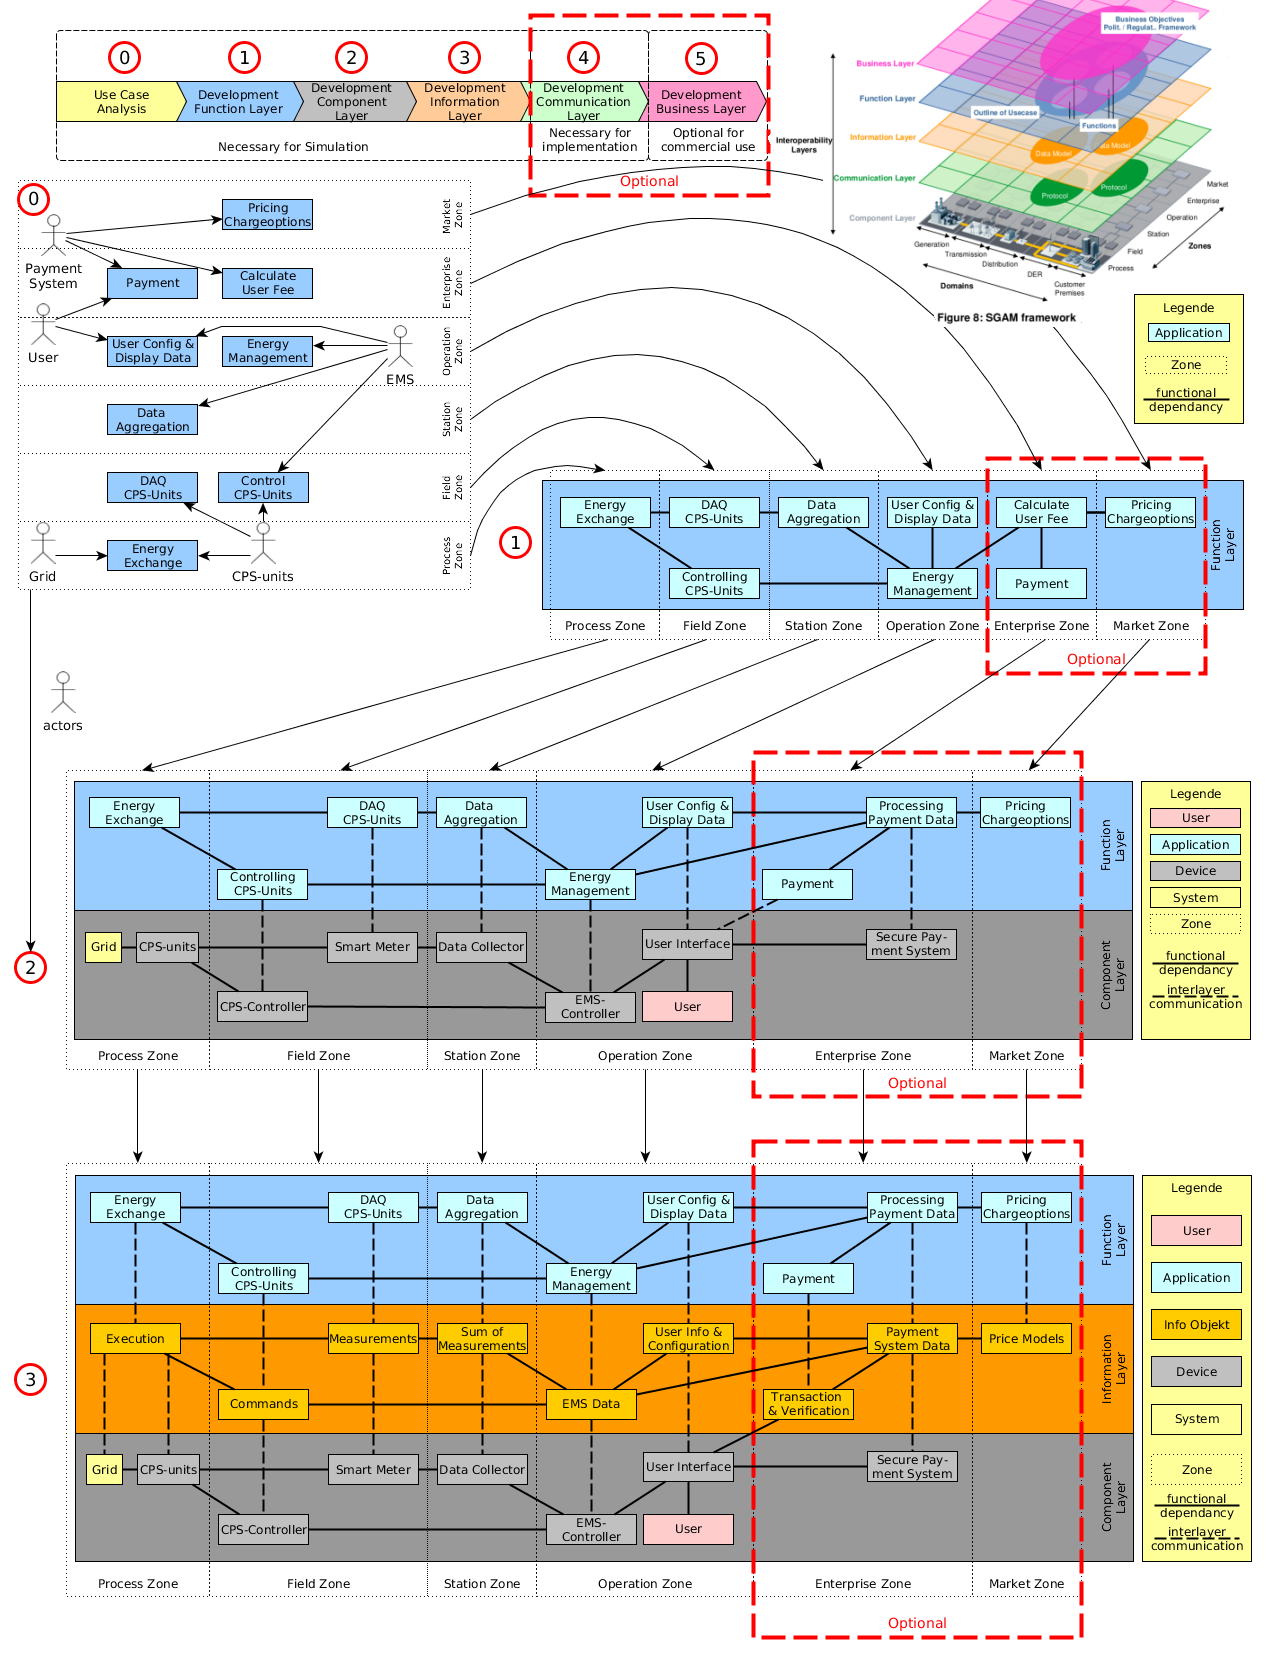
\includegraphics[width=14cm]{usecaseanalysis_overview_edit}
			\caption{Überblick der Einteilung der Energieverbundinsel in SGAM in die Ebenen Function, Information und Component, in die Domäne Customer Premises und in alle Zonen}
			\label{Abb:SGAM_map_overview}
		\end{figure} 	
        
    \begin{landscape}
        \begin{figure}[h] % NOTE REF
            \centering
            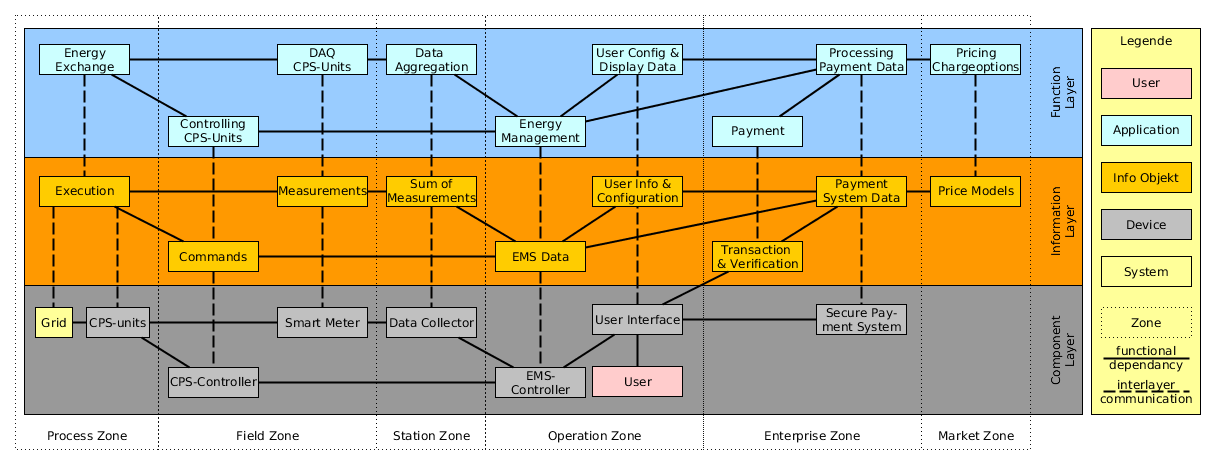
\includegraphics[width=\linewidth]{usecaseanalysis_all_total}
            \caption{Einordnung des Use Case in SGAM Ebenen Function, Information und Component über alle Zonen}
            \label{Abb:SGAM_map_all_total_big}
        \end{figure} 
	\end{landscape}